\documentclass{bioinfo}
\copyrightyear{2005}
\pubyear{2005}

\begin{document}
\firstpage{1}

\title[short Title]{A Pathvisio plugin for visualization of metabolite information}
\author[Sample \textit{et~al}]{R. Fijten\,$^{1,*}$, Egon Wilighagen\,$^{1}$ \footnote{to whom correspondence should be addressed}}
\address{$^{1}$Department of Bioinformatics, Maastricht University, Address XXXX}

\history{Received on XXXXX; revised on XXXXX; accepted on XXXXX}

\editor{Associate Editor: XXXXXXX}

\maketitle

\begin{abstract}

\section{Motivation:}
Recent developments have shown the importance of metabolomics in human systems biology research.  Given their crucial and central role as particles capturing information from all functional levels of the cell, they can provide the link between transcription and actual phenotyping. It is therefore important to develop tools that implement metabolomics data into for example pathway development tools such as Pathvisio. Pathvisio is an open source pathway development program that utilizes pathways in the WikiPathways database. A high number of these pathways contain metabolites that play a crucial role in that pathway. The plugin for metabolite information can be used to access data for these metabolites directly from within the program without using a browser. The plugin visualizes widely used IDs, molecular formula's, SMILES, InChIs and implements NMR and MS data. 

\section{Results:}
Use-case: When selecting a metabolite in pathvisio, the plugin will show a number of types of data, including predicted Mass spectrometry and Nuclear Magnetic Resonance data.

\section{Availability:}
The plugin is available on the  \href{http://pathvisio.org/wiki/PluginDocumentation}{plugin page} of the Pathvisio website
\section{Contact:} Rianne Fijten: \href{riannefijten@gmail.com}{E-mail}, \href{https://twitter.com/riannefijten}{Twitter}
\end{abstract}

\section{Introduction}
Understanding organisms, their functioning and disease are the essential building blocks of life science research. Previously, a lot of work was performed on the genome and proteome. However, the metabolome is also a vital part of cellular functioning and is most related to the phenotype, and thus an important factor in life science research.

Metabolomics is the field of research that investigates the role of groups of or separate metabolites in disease or other cellular processes. However, analysis and visualization of the data may cause problems.

Fortunately, some tools exist that can analyse and visualize metabolome data. Wikipathways is one of these tools and is an open access and open source database which contains a multitude of pathways for many different species of organisms. These pathways are created manually and are curated by the Wikipathways community. \cite{kelder} Pathvisio \cite{iersel} is a stand-alone application for computers that is based on Wikipathways and can be used to create pathways without having to use the web client. It also has additional functionalities which have been developed as Pathvisio plugins.

In order to fully incorporate metabolomics in Pathvisio data analysis, a new plugin is needed that can display information about certain metabolites from within the Pathvisio window. This will allow the researcher to immediately discover interesting properties of those metabolites and allow the researcher to compare their NMR and MS metabolite results with predicted spectra available in commonly used databases.

\begin{methods}
\section{Methods}

%1. write a plugin to visualize MS and NMR properties of metabolites
%2. using PathVisio as GUI
%3. using the CDK for cheminformatics and property prediction
%4. use HMDB voor experimental data

The plugin provides important information for the selected metabolite in Pathvisio. It has been split up into three categories. First, general information is shown, including HMDB ID, InChI and InChI key, molecular formula and the metabolite's name. Secondly, linkouts to MS spectra and NMR spectra from the HMDB database are provided. Finally, carbon NMR chemical shifts have been calculated and are shown in the plugin window.

Several databases have been used to collect and calculate the many important metabolite properties.The HMDB database \cite{hmdb} was used to import imformation such as predicted NMR and MS spectra. Moreover, the Chemical Identifier Resolver was used to retrieve the InChI ID and InChI key. Furthermore, the NMR chemical shifts were calculated using the Chemistry Development Kit  \cite{cdk}. Finally, the BridgeDb framework implemented inside Pathvisio was used to obtain basic metabolite information such as the metabolite name and HMDB ID \cite{bridge}.

\end{methods}

\begin{figure*}[!tpb]%figure1
\centerline{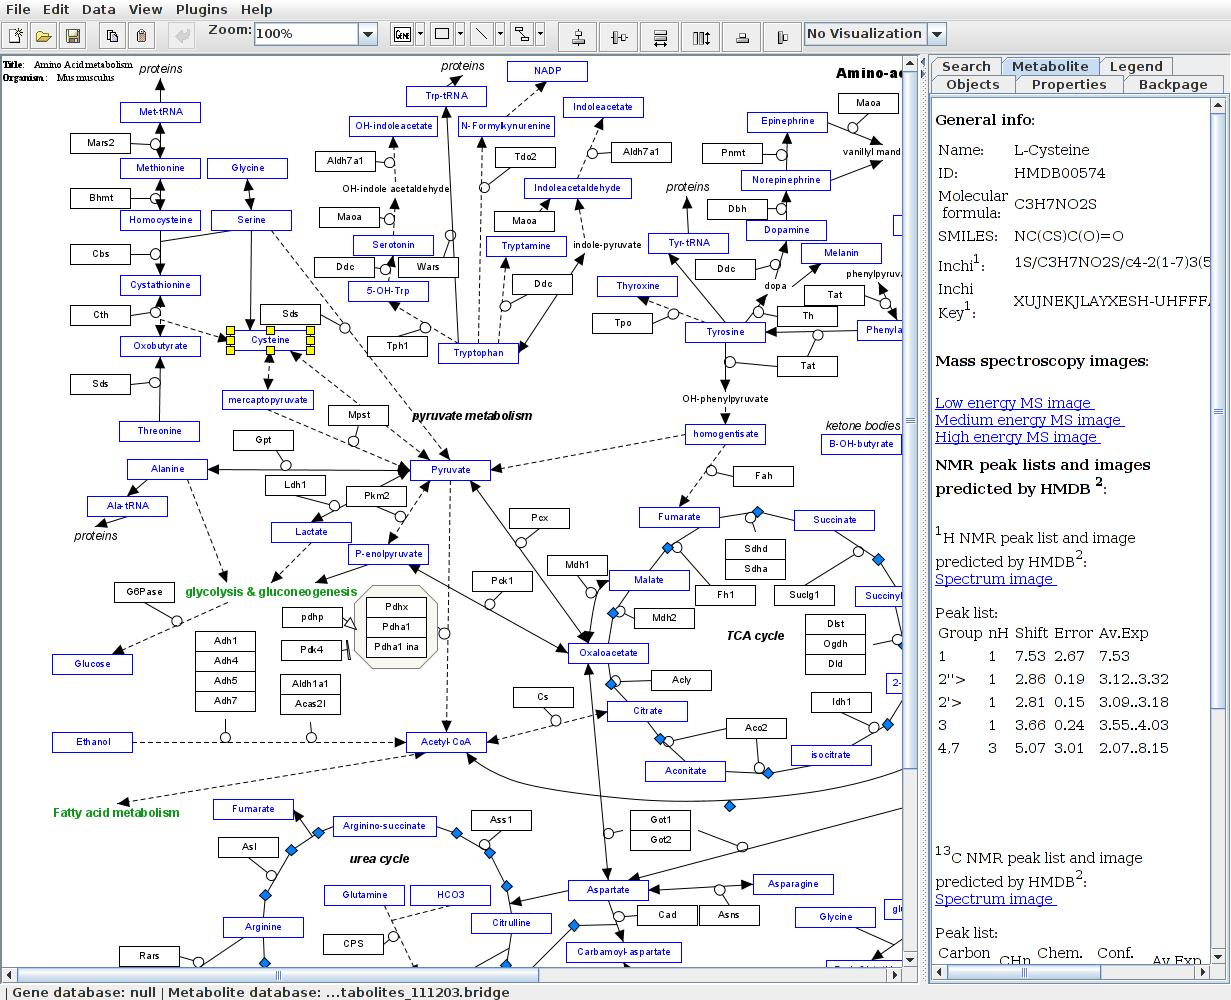
\includegraphics[width=10cm]{figure1.png}}
\caption{The pathvisio window with a pathway on the left, and the plugin on the right. The metabolite cysteine was selected, and all available information at the time is visible.}\label{fig:01}
\end{figure*}

%\begin{figure}[!tpb]%figure2
%\centerline{\includegraphics{fig02.eps}}
%\caption{Caption, caption.}\label{fig:02}
%\end{figure}

\section{Discussion}
Some things might cause problems using this plugin. Preferably, the plugin should also show experimental MS and NMR data in order to complement the predicted properties and allow comparison between the two.

Another problem that the plugin faces is that it is limited by the metabolite identifier that are used in the Pathvisio pathways. Additionally, not all metabolites are well-defined in structure or function, which might lead to misinterpretation by CDK. 

The biggest problem is the fact that the HMDB database was updated during the project. The new version does not allow prediction of the url. Therefore the parts of the plugin that originated from the HMDB database are currently not working.

\section{Conclusion}

Summary of the plugin and what it can do.
The plugin is a good tool to immediately provide users with the metabolite information they require. Link outs to the HMDB database will give enhanced functionality and the possibility for the used to easily find even more information than the plugin provides.
Future development
\begin{itemize}
    \item Visualization of experimental NMR and MS spectra
    \item Overview of pathway metabolites and their properties
    \item Addition of figures showing spectra to the tables
\end{itemize}

\bibliographystyle{natbib}
%\bibliographystyle{achemnat}
%\bibliographystyle{plainnat}
%\bibliographystyle{abbrv}
%\bibliographystyle{bioinformatics}
%
%\bibliographystyle{plain}
%
\bibliography{bioinf}

\end{document}